
\documentclass[preprint,12pt]{elsarticle}

\usepackage[spanish]{babel}
\usepackage{amssymb}
\usepackage{graphicx}
\usepackage{lineno}
\usepackage[utf8]{inputenc}
\usepackage{url}
\usepackage{natbib} 
\usepackage{amsmath} 
\usepackage{amssymb} 

\begin{document}
	
	\begin{frontmatter} 

		\title{\huge MÁQUINAS VIRTUALES VS CONTENEDORES}
		
		\author{Estrella Palacios, Katherine Lizbeth              	(2016056193))}
		\author{Gonzales Cave, Angel Gabriel              	(2017057861))}
		\author{Porlles Carrillo, Diego Armando	         	(XXXXXXXXXX))} %CAMBIAR CODIGO 
		\author{Quispe Mamani, José Luis             		(XXXXXXXXXX))} %CAMBIAR CODIGO 
		\address{Escuela Profesional de Ingeniería de Sistemas}
		\address{Universidad Privada de Tacna}
		\address{Tacna, Perú}
		
%% ABSTRACT --------------------------------------------------------------------------------------------------------------------

		\begin{abstract}
		


		\end{abstract}

%% ----------------------------------------------------------------------------------------------------------------------------------

	\end{frontmatter}

%% RESUMEN ---------------------------------------------------------------------------------------------------------------------

\section{Resumen}



%% ----------------------------------------------------------------------------------------------------------------------------------


%% INTRODUCION ----------------------------------------------------------------------------------------------------------------

\section{Introducción} 





%% ----------------------------------------------------------------------------------------------------------------------------------


%% MARCO TEÓRICO ------------------------------------------------------------------------------------------------------------

\section{Marco Teórico}

%% PRIMERA SUBSECCION 

\subsection {\textbf{A}}

\subsubsection{\textbf{A1}}

EDITAR\\

%%Ejemplo de cita
\cite{Gartner} 

\begin{itemize}
	\item x
	\item y
	\item z
\end{itemize}

\subsubsection{\textbf{A2}}

EDITAR\\

\subsubsection{\textbf{A3}}

EDITAR\\


%% SEGUNDA SUBSECCION

\subsection{\textbf{B}}

\subsubsection{\textbf{B1}}

EDITAR\\

%% Ejemplo de inclusión de imagen
\begin{figure}[htb]
	\begin{center}
		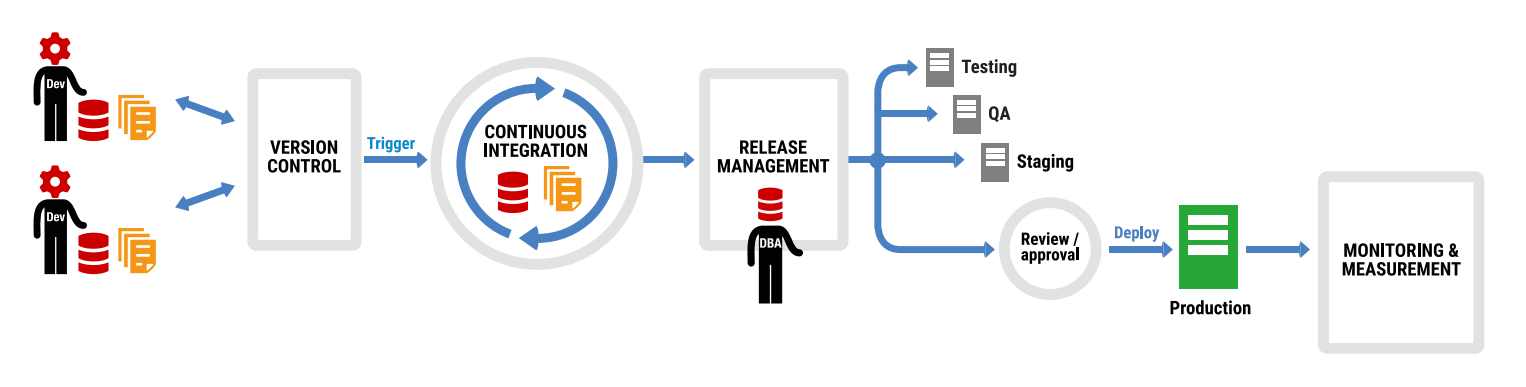
\includegraphics[width=14cm]{./IMAGENES/basededatos_1} 
		\caption{Incluyendo la base de datos en DevOps}
	\end{center}
\end{figure}

\subsubsection{\textbf{B2}}

EDITAR\\

%% TERCERA SUBSECCION
\subsection{\textbf{C}}

\subsubsection{\textbf{C1}}

EDITAR\\

\begin{itemize}

\item x
\item y
\item z

\end{itemize}
\subsubsection{\textbf{C2}}

EDITAR\\


%% ----------------------------------------------------------------------------------------------------------------------------------
 


%% ANÁLISIS ( APLICACIÓN ) ---------------------------------------------------------------------------------------------------

\section{Análisis}

\subsection{\textbf{Análisis 1}}
EDITAR\\

\subsection{\textbf{Análisis 2}}
EDITAR\\

\subsection{\textbf{Análisis 3}}
EDITAR\\

\subsection{\textbf{Análisis 4}}
EDITAR\\

%% ----------------------------------------------------------------------------------------------------------------------------------


%% CONCLUSIONES ---------------------------------------------------------------------------------------------------------------

\section{Conclusiones}

\begin{itemize}

\item Conclusion 1 : \\

\item Conclusion 2 : \\ 

\item Conclusion 3 : \\ 

\item Conclusion 4 : \\ 
\end{itemize}

%% ----------------------------------------------------------------------------------------------------------------------------------

%%  REFERENCIAS BIBLIOGRÁFICAS ------------------------------------------------------------------------------------------
	
	\newpage
	
	\bibliographystyle{apalike} 	%ESTILO
	\bibliography{BIBLIOGRAFIA}	 
	
	
\end{document}
